% To teach: curation, presentation, feedback

% test account: labsmbatest, wharton1
% See {\it Notebook} 2008-6-4 pages 6--7,  2008-7-15 pages 38--40 and {\it Daybook}2008-8-14, pages 47--8.
% On the cosine measure of similarity:
% http://www.miislita.com/information-retrieval-tutorial/cosine-similarity-tutorial.html


% Citation: "The outbreak of cooperation among success-driven
% individuals under noisy conditions." By Dirk Helbing and Wenjian
% Yu. Proceedings of the National Academy of Sciences, Vol. 106, No. 8,
% Feb. 23, 2009.

% \begin{figure}[htbp] %  figure placement: here, top, bottom, or page
%    \centering
%    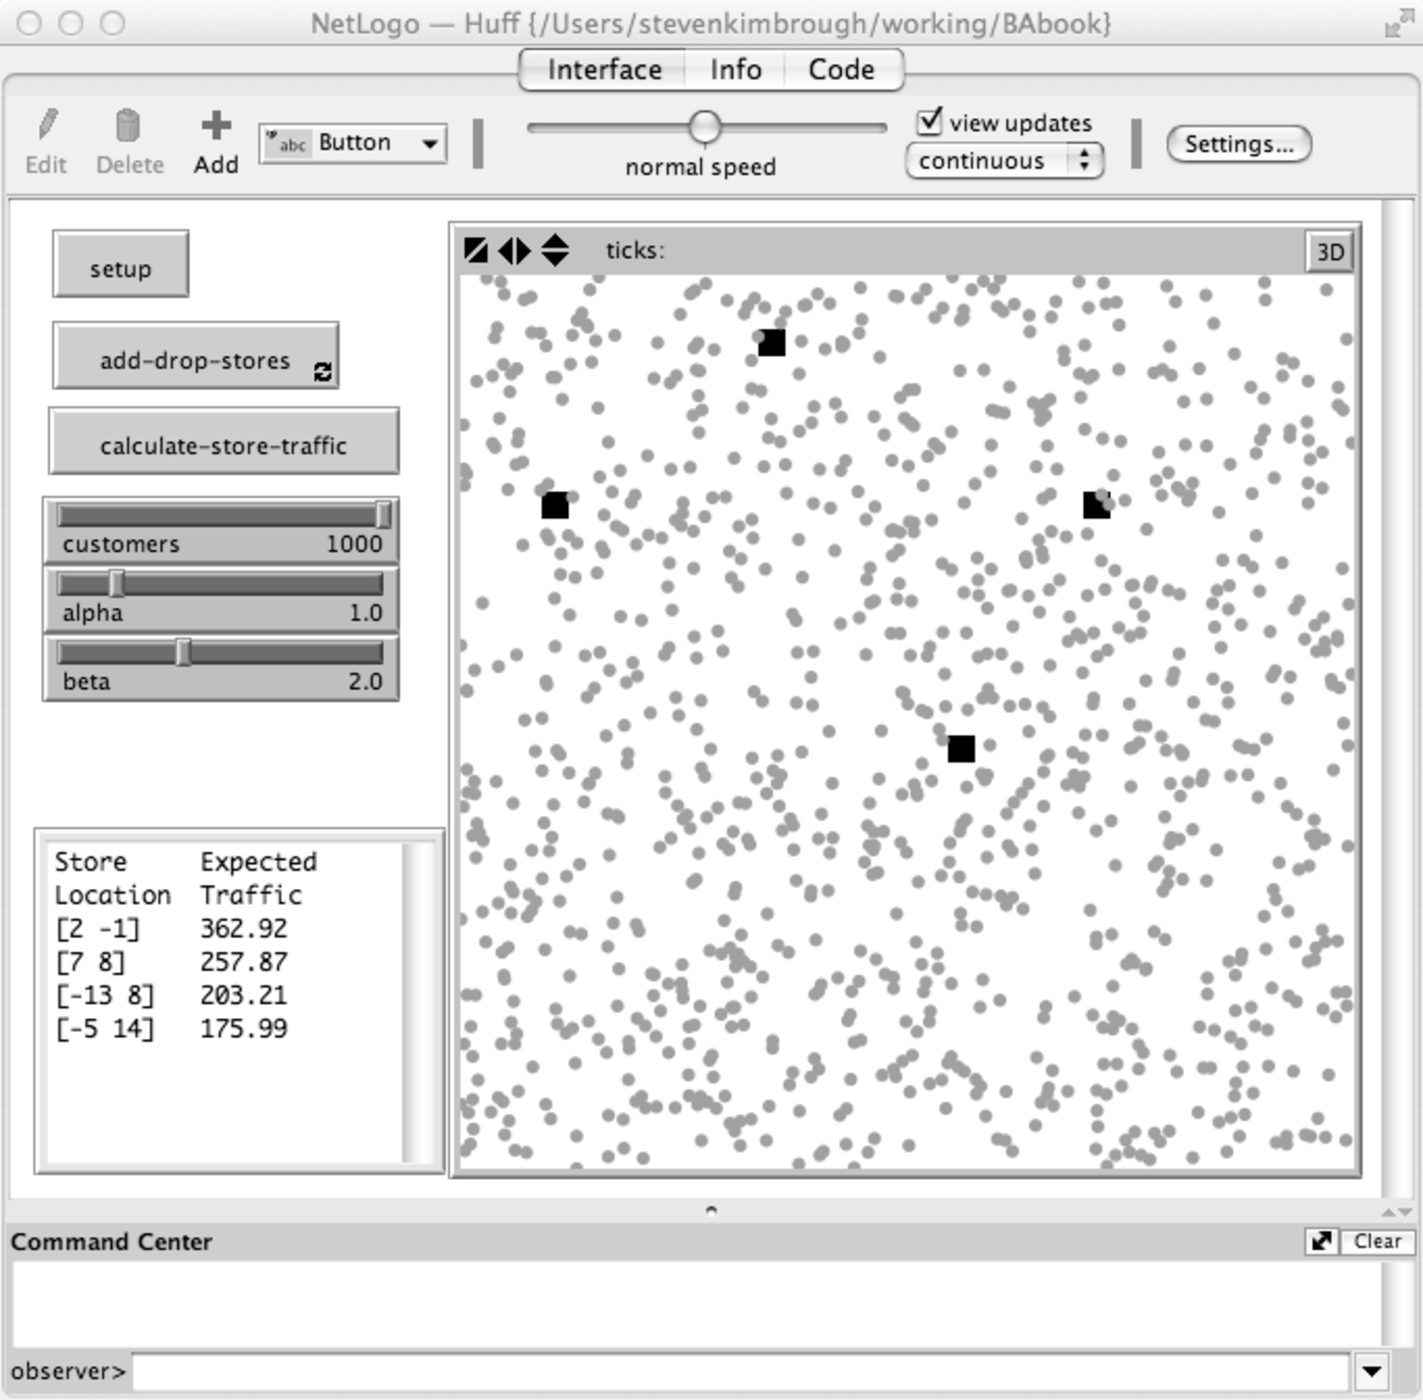
\includegraphics[width=\textwidth]{figures/HuffPatches.pdf}  
%    \caption{Huff, a NetLogo implementation of Huff's model.} % using random-seed 22478
%    \label{fig:huffnlogo}
% \end{figure}

\def\noop#1{}
\def\mlb{MATLAB}
\def\figtop{\rule{\textwidth}{0.5mm}}
\def\figbot{\rule{\textwidth}{0.5mm}}
%%%%%%%%%%%%%%%%%%%%%%%%%
   



 \def\year{2016}
 \def\lastclass{Wednesday, April 29, \year}
%  \def\matlabcasedue{9 p.m. on Monday, March 30, 2015}
%  \def\groupassignmentdue{5 p.m. on Tuesday, May 5, 2015}
%  \def\pythoncasedue{5 p.m. on Thursday, May 7, 2015}
% \def\nis{../../../books/RobustDecisionMaking/NewImages/}
% \def\mlb{MATLAB}
% \def\mb{{\it DAMbook}}
\def\noop#1{}
\def\place{TBA}
\def\figtop{\rule{\textwidth}{0.5mm}}
\def\figbot{\rule{\textwidth}{0.5mm}}
\noop{
\section{Readings}
\section{Lecture notes}
\section{Exercises}
\section{In class assignments}
\section{Case assignments}
  }
 
  
\newtheorem{exercise}{Exercise}
\documentclass[11pt]{book}
\makeindex
\usepackage{url}
\usepackage{palatino}
%
\usepackage{hyperref}
\usepackage{color}
\usepackage{amssymb}

\usepackage{makeidx}
%\usepackage{geometry}
%\geometry{textwidth=6.5in}

\usepackage{rotating} % for sideways and sidewaystable, etc. environments
% the following package, when present, lets the figures and tables orient oppositely on even and odd pages
\usepackage{lscape} 
\usepackage{natbib}

%%%%%% From KAPSARC document, for funny characters
\usepackage{etoolbox}
\usepackage{pifont}
%%%%%%%%%%%%%%%%%%%%%%%%%%%%%

\makeindex
\newcount\draft
\draft=1
\newcount\instructor
\instructor=1
\newcount\answers
\answers=1
%%%%%%%%%%%%%%%%

\begin{document}

%\index{BMI!|see{body mass index}}

\pagenumbering{roman}
\setcounter{secnumdepth}{5}
\setcounter{tocdepth}{2}
\frontmatter
%\nocite{*}
%
\pagestyle{empty}
\centerline{\Huge DOID 325: Thinking with Models}
\vskip 12 pt
\centerline{\Large Spring 2016, \place}
\vskip 30 pt
\centerline{\Large Teaching Notes (and Class Record)}
\vskip 35 pt
\centerline{\Large Steven O. Kimbrough}
\vskip 35 pt
\centerline{Draft: \copyright\ \today}

\ifnum\draft=1
\vfill
{\footnotesize
\noindent\verb+$Id: TwM-class-s2016-teaching-notes-master.tex 4950 2015-09-13 18:31:27Z sok $+
}
\fi
% \newpage

% \noindent Steven O. Kimbrough, %103 Bentley Avenue, Bala Cynwyd, PA 19004--2805. 
% Tel: (215) 898-5133.  Fax: (215) 898-3664. Email: kimbrough@wharton.upenn.edu. Web: %{\tt http://opim.wharton.upenn.edu/\symbol{126}sok/}.
% \url{http://opim.wharton.upenn.edu/~sok/}

\newpage
\pagestyle{plain}
\tableofcontents

%
\listoffigures

%
\listoftables

%\chapter{Executive Summary}
\chapter{Preface}

\mainmatter
\pagenumbering{arabic}
%
\pagestyle{headings}

%%%%%%%% Class 1, Introduction  %%%%%%%%%%%
\chapter{Class 1}

\chapter{Class 2}

\chapter{Class 3}

\chapter{Class 4}

\chapter{Class 8: W\&R, chapter 3, Segregation}

\section{Teaching Notes (about 20 minutes)}

Focus now on some programming techniques.
\begin{enumerate}
\item Page 132: \texttt{n-of number patches} then \texttt{sprout}.

\texttt{n-of <agentset>} is a general approach to obtaining an agentset of size \texttt{number} from another agentset. The returned agentset has no duplicates.  

\texttt{sprout} is a command to a patch, causing it to create turtles on top if. Works for breeds of turtles, too.

\item Page 133: \texttt{count (turtles-on neighbors)}. Go through this. We are in a turtle context \ldots 
\texttt{(turtles-on neighbors)} returns an agentset of turtles with the property that they are on the \texttt{neighbors} of the current turtle. Nice, elegant construction.

\item Page 133: \texttt{with} qualities an agentset and can be arbitrarily complex. Note the syntax. Can have arbitrary boolean combinations inside \texttt{[ \ldots ]}.

\item The book discusses \texttt{update-turtles} but not the enclosing procedure \texttt{update-variables}. Important to see how this works: turtles are moved individually; once all the turtles are moved, the updating happens. Discuss: Why is this necessary? This is why we need a \texttt{happy?} attribute.

\item Page 135: \texttt{set color (item (random number-of-ethnicities) colors)}. OK, explain how it works. Now, what if we want the ethnicities not to be equi-probable? What can we do?

\item Page 136: \texttt{random \%-similar-wanted}. Discuss how this works. Note it's a bit odd. What about using \texttt{random-normal}? How would that work?  Discuss other probability distributions supported by NetLogo and what they might be good for.
\end{enumerate}

\section{Exercises (about 40 minutes)}

Form groups of 3 (2 or 4 as necessary). Discuss and write down and load to Canvas responses to the following.

\begin{enumerate}
\item Add agents that don't care, that is, are happy with no neighbors of their own color. Have them move occasionally. Develop a slider for the number of don't care agents of each color.

Explore the resulting model. How does it behave? Compare with the original model and the extensions from the book.

\item Percent similar is a key measure of performance (MoP) of the system as modeled. It only looks at immediate neighborhoods. Use \texttt{in-radius} to develop a more flexible MoP that looks at neighborhoods of arbitrary size (to be indicated by a slider). Be careful to count only \texttt{other} turtles.
\end{enumerate}

\section{Class Discussion (about 20 minutes)}

Discuss the exercises with the entire class. What did people do?

To the extent there is time: Discuss what would be needed to get a reasonably accurate and well calibrated segregation model.

\chapter{Class 9: W\&R, chapter 3, El Farol}

\section{Teaching Notes (about 20 minutes)}

Focus now on some programming techniques and on the El Farol model itself.
\begin{enumerate}
\item Do a walkthrough of the El Farol code, explaining how it works.
\item Pages 143--4: Discuss \texttt{turtles-own} (again) and step through the handling of \texttt{reward}.
\item Page 145: Discuss \texttt{scale-color} and how it works.
\item Work through histograms carefully and explicitly.
\end{enumerate}

\section{Exercises (about 40 minutes)}

Form groups of 3 (2 or 4 as necessary). Discuss and write down and load to Canvas responses to the following.

\begin{enumerate}
\item Write code to report the three best strategies and the three worst strategies, so that we can look at them. What do you find?
\item Do exercise 32 on page 155 of the book.

\item Implement a win-stay/lose-shift strategy and put it into the model.
\end{enumerate}

\section{Class Discussion (about 20 minutes)}

Discuss the exercises with the entire class. What did people do?





%%
%\input chapters/introduction.tex
%
%\part{Programming NetLogo}
%%%%%%%%% Class 2, NetLogo Overview and working with patches  %%%%%%%%%%%
%\input chapters/intro-patches/intro-patches.tex
%
%%%%%%%%% Class 3, Working with turtles  %%%%%%%%%%%
%\input chapters/intro-turtles/intro-turtles.tex
%
%%%%%%%%% Class 4, Intro Plotting  %%%%%%%%%%%
%\input chapters/intro-plotting/intro-plotting.tex
%
%\part{Modeling Examples}
%
%\input chapters/converse.tex
%
%\input chapters/huff.tex
%
%\input chapters/gdp/groupdecisionprediction.tex
%%%%%%%%%%%%%%%%%%%%
%\part{Exploratory Modeling} %{Reasoning with Models} % with thanks to Steve Bankes


\appendix

%\ifnum\draft=1
%\input chapters/dev-notes.tex
%\fi

\backmatter
\addcontentsline{toc}{chapter}{References}
%
\bibliographystyle{apalike} %{amsalpha} %plain}
\bibliography{../../sok,../../union}

\addcontentsline{toc}{chapter}{Index}
%\input 311s2015-teaching-notes-master.ind

\end{document}




% \addcontentsline{toc}{chapter}{References}
% %
% \bibliographystyle{apalike} %{amsalpha} %plain}
% \bibliography{../../sok,../../union}

% \addcontentsline{toc}{chapter}{Index}
% %
% \input 311s2014-teaching-notes-master.ind
% \end{document}

